% getikz enable true
%! Available geTikZ-commands:
% getikz library calc,fit,backgrounds
%! % getikz header <header e.g. \usepackage commands>
% getikz path ../..
%! For a description of these and other commands have a look at
%! https://gitorious.org/getikz/pages/Commands

\def\venue{red}
\def\social{blue}
\def\location#1#2{\draw[line width=2,color=#2,opacity=0.7] (#1) circle[radius=0.025]; }
\def\loclabel#1#2#3{\node[anchor=#1,outer sep=6,fill=white,fill opacity=0.5,text opacity=1,rounded corners] at (#2) {\bf #3}; }

\ifx\imgtitle\undefined
\def\imgtitle#1#2#3{}
\fi

\begin{tikzpicture}

  % 21cm
  \pgfmathsetmacro{\scale}{\linewidth/1190bp}
  \pgfmathsetmacro{\backscale}{1190bp/\linewidth}

  \begin{scope}[scale=\scale]

    % 1190bp scaled manually
    \begin{scope}[on background layer]
      \node[outer sep=0,inner sep=0] (map) {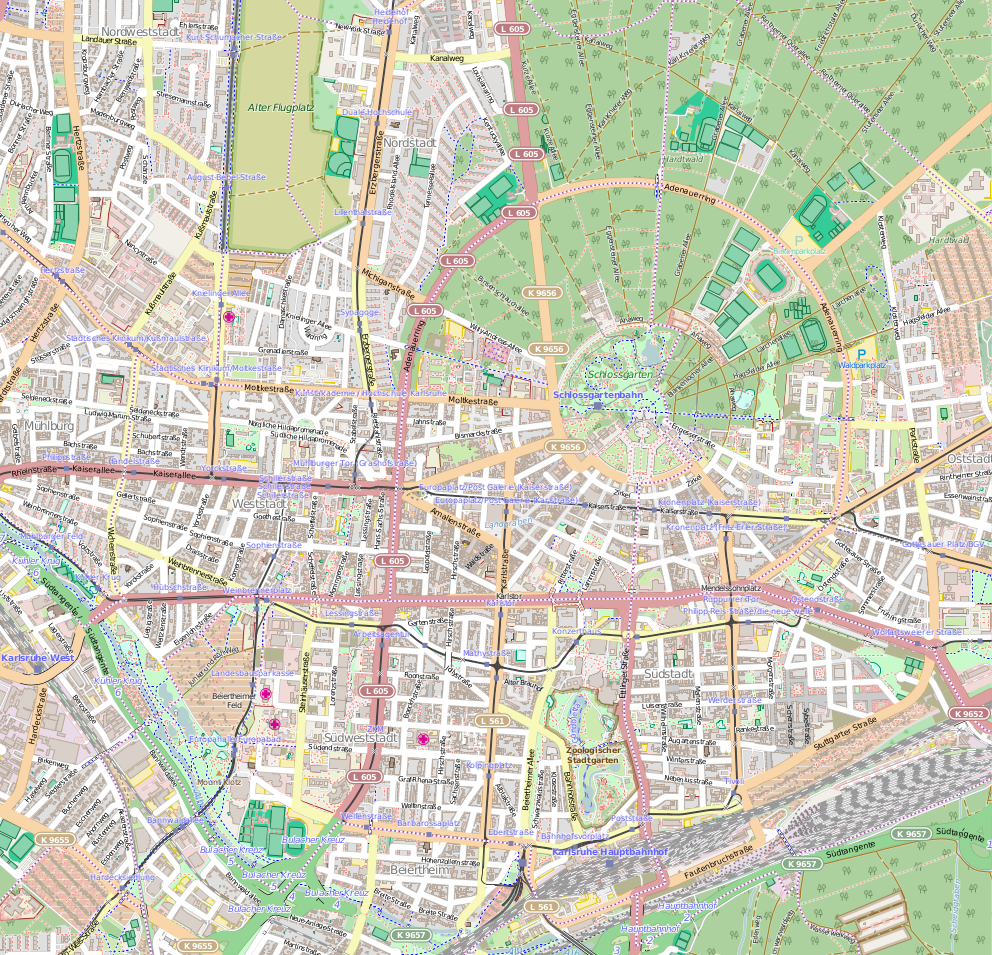
\includegraphics[width=\linewidth,trim=0 100 0 100,clip]{images/map/osm-ka-low.png}};
    \end{scope}

    \node[anchor=center,coordinate] (center) at (6.28cm,2.78cm) {};
    \node[anchor=center,coordinate] (615m) at (14.85cm,2.78cm) {};

    \begin{scope}[shift=(center),scale=1000*(14.85-6.28)/615]
      \node[anchor=center,coordinate] (schloss) at (0,0) {};
      \node[anchor=center,coordinate] (zoo) at (-0.19,-0.95) {};
      \node[anchor=center,coordinate] (hbf) at (-0.2,-1.33) {};
      \node[anchor=center,coordinate] (zkm) at (-0.9,-0.88) {};
      \node[anchor=center,coordinate] (dhbw) at (-0.84,+0.88) {};
      \node[anchor=center,coordinate] (campus) at (+0.35,-0.2) {};
      \node[anchor=center,coordinate] (waldparkplatz) at (+0.68,+0.18) {};
      \node[anchor=center,coordinate] (karlshs) at (-0.46,-0.5) {};
      \node[anchor=center,coordinate] (z10) at (+0.46,-0.36) {};
      \node[anchor=center,coordinate] (akk) at (+0.45,-0.2) {};
      \node[anchor=center,coordinate] (hadiko) at (+0.82,0.4) {};
      \node[anchor=center,coordinate] (jugendherberge) at (-0.5,+0.1) {};
      \node[anchor=center,coordinate] (info) at (+0.68,+0.0) {};
      \node[anchor=center,coordinate] (markt) at (-0.02,-0.3) {};

      \location{schloss}{\social}
      \loclabel{south}{schloss}{Castle and Parc}
      \location{zkm}{\venue}
      \loclabel{east}{zkm}{ZKM}
      \location{karlshs}{\venue}
      \loclabel{north}{karlshs}{Karlshochschule}
      \location{campus}{\venue}
      \loclabel{south}{campus}{KIT/University}
      \location{dhbw}{\venue}
      \loclabel{west}{dhbw}{DHBW}
      \location{z10}{\social}
      \loclabel{north}{z10}{Z10}
      \location{akk}{\social}
      \loclabel{west}{akk}{AKK}
      \location{jugendherberge}{\social}
      \loclabel{north}{jugendherberge}{Youth Hostel}

      %\location{zoo}{\social}
      %\loclabel{east}{zoo}{Zoo}

      \location{markt}{\social}
      \loclabel{north}{markt}{City Center}

      \location{info}{\venue}
      \loclabel{south}{info}{CS Department}

      \location{hbf}{\social}
      \loclabel{south}{hbf}{Main Station}



      \node[coordinate] (legend) at ($(map.south west)+\scale*(2ex, 1.8em)$) {};
      \node[coordinate] (legend-out) at ($(legend)+(1,0)$) {};

      \begin{scope}
        \draw[line width=2pt,opacity=0.7,line cap=round] ($(legend) + (0, 0.025)$) -- (legend) -- node[above,opacity=1,inner sep=0,yshift=2pt] (kmlabel) {1\,km} ++(1, 0) -- ++(0, 0.025);

        \node[anchor=south west,inner sep=0pt] (copyright) at ($(legend) + \scale*(0, -1em)$) {\imgtitle{OpenStreetMap contributors}{Map of Karlsruhe}{CC BY-SA 2.0, overlays added, \url{http://www.openstreetmap.org/copyright}}};
      \end{scope}

      \begin{scope}[on background layer]
        \node[fit=(legend) (legend-out) (kmlabel) (copyright),fill=white,opacity=0.8,rounded corners] {};
      \end{scope}

    \end{scope}
  \end{scope}

\end{tikzpicture}
